\documentclass[a4paper,11pt]{article}
\usepackage[T1]{fontenc}
\usepackage[utf8]{inputenc}
\usepackage{lmodern}
\usepackage[french]{babel}
\usepackage{graphicx}
\usepackage{cite}
\usepackage{hyperref}
\usepackage{array}

\title{%
  Rapport d'avancement thèse ACSEL \\
  \large Comité de Suivi Individuel 09/2018 \\ % Subtitle
  \large \textit{Sous la direction de David Defour, MCF HDR 27e et Bijan Mohammadi, Pr, 26e}}
\author{Christophe Pont}

\graphicspath{{illustrations/}}

\begin{document}

\maketitle
\tableofcontents

%\begin{abstract}
%\end{abstract}

%%% PRESENTATION
\section{Présentation}

% PRESENTATION PERSONNELLE
\subsection{Présentation personnelle}
Après l’obtention d’un Bac S spé maths (mention bien) à Toulouse, j’ai intégré un DUT Informatique, que j'ai obtenu avec la mention Bien. Mon cursus s’est prolongé à Polytech Montpellier, où j’y ai obtenu mon diplôme d’ingénieur en Informatique et Gestion (mention Bien). Durant cette formation, j’ai pu réaliser un stage anglophone dans un laboratoire de bioinformatique à l’université d’Ottawa, au Canada. Ce premier contact avec la recherche m’a incité à démarrer un doctorat, en octobre 2017, après deux ans en tant qu’ingénieur logiciel dans une grande entreprise de service informatique (SSII). L’idée était d’harmoniser mon orientation avec mon attrait pour la science, en particulier l’informatique et les mathématiques. C’est pourquoi je me suis dirigé vers le laboratoire LAMPS, et ai démarré mon doctorat sous la direction de David Defour, HDR, 27e afin de démarrer une thèse mêlant ma compétence informatique avec mon attrait pour les mathématiques : le tout, dans un contexte écologique qui me tient à cœur. J’aspire à continuer ma carrière dans la recherche, qui sait peut-être en tant que maître de conférence.

% PRESENTATION THESE
\subsection{Contexte}
Le contexte dans lequel se place mon sujet de thèse est double.
D’un côté, on s’intéresse à l’\textbf{arithmétique flottante}. \\
Les nombres flottants peuvent se définir comme une discrétisation des nombres réels. 
Le Standard IEEE 754\cite{zuras2008ieee} définit 3 entiers $(s,e,m)$ pour représenter nombres flottants (en l'occurence $s$ étant le bit de signe, $e$ l'exposant et $m$ la mantisse). Il fournit aussi des \textbf{formats}, qui définissent la façon dont chaque nombre flottant est \textbf{encodé}. On peut citer le format simple précision, le format double précision etc. \\
\begin{figure}[b]
  \begin{center}
    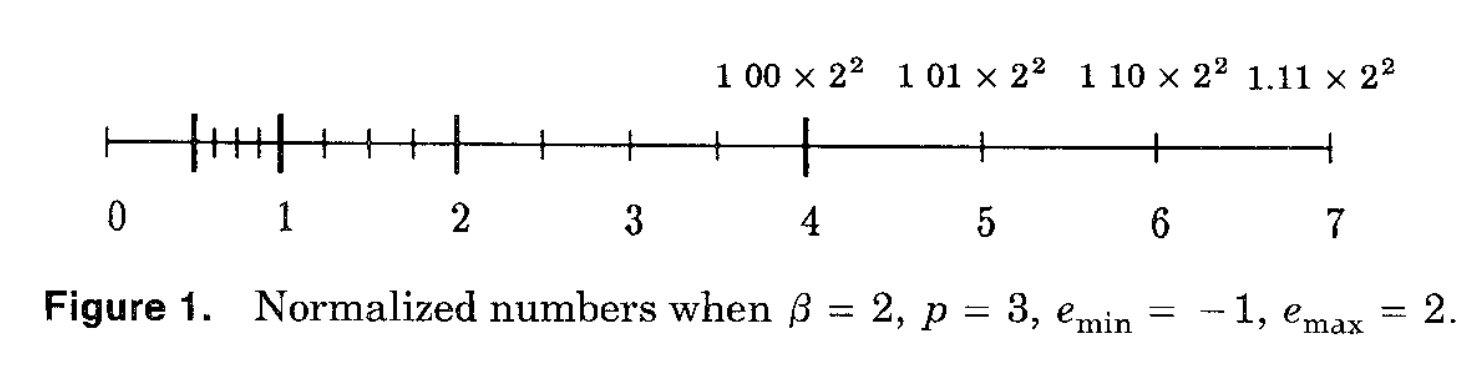
\includegraphics[width=12cm]{Floating_point_numbers_discretization}
    \caption{Exemple de discretisation des nombres réels en nombres flottants. Source : \cite{goldberg1991every}}
    \label{discretization}
  \end{center}
\end{figure}
Prenons l'exemple d'une telle discrétisation (Figure ~\ref{discretization}) selon les paramètres suivants : $\beta=2, p=3, e_{min}=-1,e_{max}=2$, avec $\beta$ la base, $p$ la précision (soit le nombre de bits de la mantisse), $e_{min}$ l'exposant minimal et $e_{max}$ l'exposant maximal.
Sur l'exemple, on voit bien que $1,25$ est représentable ($1.01*2^{0}$), de même que $3$ ($1.10*2^{1}$). Bien que la somme de ces deux réels donne $3,25$, la somme flottante de ces deux nombres flottants donne elle $3$ (après arrondi), car $3,25$ n'est pas représentable exactement dans ces conditions.

Malgré la définition d'un standard, l'arithmétique flottante est soumise à de multiples erreurs. On pense notamment aux \textbf{erreurs d'arrondi}, comme dans le cas cité ci-dessus où $3,25$ a dû être arrondi à $3$, entraînant la \textit{perte} de $0,25$. Mais on peut aussi citer les \textbf{erreurs de cancellation}, qui surviennent lorsque l'on soustrait deux grandes valeurs très proches l'une de l'autre, révélant la perte de nombre significatifs lors de précédents calculs. \\ % TODO exemple.
Hors, lorsque l’on simule un modèle qui comprend de nombreux calculs (super calculateurs, vastes simulations à exécution longue), les différentes erreurs s’accumulent, se combinent, et finalement affectent le résultat.

Le deuxième volet de ma thèse porte sur ce domaine, celui de la \textbf{recherche d'erreurs numériques dans les programmes}.
Le cas d’étude de ma thèse porte sur les modèles et simulations de \textbf{Gladys}\footnote{\url{http://www.gladys-littoral.org}}.
Gladys est un réseau international de littoralistes en méditerranée, regroupant de nombreux chercheurs dans le domaine du littoral.
Ils ont établi de nombreux modèles pour décrire les phénomènes afférents à leur activité, notamment le phénomène \textbf{d’évolution du trait de côte}.
L’implémentation informatique de ce modèle sera le sujet d’étude de ma thèse (un code volumineux en C et Fortran). Il prend des données en entrée et réalise sa simulation. C'est ici que viendra se placer mon travail. Le principe recherché est de \textbf{compiler} le programme, puis d’en produire une analyse visant à suivre et quantifier les erreurs liées à l’arithmétique flottante.

%modèle sur lequel a travaillé Bijan  [ accrétion, érosion ]
%les résultats subissent différents types d’erreurs [EDP, on dérive en fonction du temps, les erreurs peuvent s’accumuler/se combiner]
%objectif : quantifier l’erreur informatique, numérique

\subsection{État de l’art}

On peut distinguer deux catégories d'initiatives existantes dans le domaine : les démarches visant à \textit{limiter} l’effet des erreurs (on peut citer les sommations compensées\cite{Demmel2006ErrorBF}, Salsa\cite{damouche2016amelioration}...), et celles visant à quantifier et mesurer les erreurs.
Ma thèse fait écho à cette deuxième approche.
La riche littérature existante fait état de nombreux outils pouvant réaliser cette analyse. Chacun dispose cependant de différentes entrées (programmes, modèles, binaires…), et différentes contraintes.
On s’intéresse ici à deux approches probabilistes en particulier : la méthode CESTAC\footnote{\underline{C}ontrole et \underline{E}stimation \underline{S}tochastique des \underline{A}rrondis de \underline{C}alculs}, et l’arithmétique de Monte Carlo\footnote{ou MCA (\underline{M}onte \underline{C}arlo \underline{A}rithmetic)}.
La méthode CESTAC\cite{pichat1993ingenierie} utilise un grand nombre de tirages pour approximer efficacement le nombre de bits significatifs du résultat.
DSA\footnote{\underline{D}iscrete \underline{S}tochastic \underline{A}rithmetic}\cite{vignes2004discrete}, basée sur CESTAC, redéfinit quant à elle les opérateurs relationnels pour effectuer chaque opération $N$ fois, en changeant aléatoirement le mode d’arrondi (et définit aussi les notions de nombre stochastique et de zéro stochastique).
Enfin, CADNA\footnote{\underline{C}ontrol of \underline{A}ccuracy and \underline{D}ebugging for \underline{N}umerical \underline{A}pplication}\cite{jezequel2008cadna} implémente DSA pour $N=3$, où les deux premiers modes d’arrondis sont choisis aléatoirement, et où le troisième est différent du second. \\
Parallèlement, MCA\cite{parker1997monte} permet une analyse de sensibilité, en utilisant notamment un \textit{arrondi randomisé} pour ajouter du bruit aux nombres flottants, à l'aide d'une variable aléatoire uniformément distribuée, afin de quantifier et compenser les erreurs d'arrondi notamment.
Finalement, Verificarlo\cite{denis2015verificarlo} est une implémentation de MCA utilisant LLVM\footnote{\url{https://llvm.org/}} pour la portabilité.
On citera aussi FPANR\footnote{\underline{F}loating-\underline{P}oint \underline{A}daptive \underline{N}oise \underline{R}eduction}\cite{defour2018fp}, encodage proposé par David Defour, qui comme on va le voir encode astucieusement la précision dans la mantisse.

%MCA et DSA : deux méthodes probabilistes vérifier précision arithmétique
%(Verificarlo prétend que les hypothèses de CESTAC ne tiennent pas : “je n’ai pas le recul pour m’exprimer sur le sujet”)

%CESTAC : Controle et Estimation Stochastique des Arrondis de Calculs
%DSA : Discrete Stochastic Arithmetic
%CADNA : Control of Accuracy and Debugging for Numerical Application
%SAM : Stochastic Arithmetic in Multiprecision
%MCA : Monte Carlo Arithmetic
%FP-ANR : Floating-Point Adaptive Noise Reduction

%Analyse statique

\section{Travail réalisé}

\subsection{Arrondi randomisé }
Nous avons utilisé l'arrondi randomisé, inspiré du \textit{round\_ random\_nearness} de MCA. 
La motivation est simple : à la fois tracer les erreurs en utilisant notamment l'écart type des tirages, ainsi que \textit{compenser statistiquements} les erreurs d'arrondis à l'aide du grand nombre de tirage.
Le principe est le suivant : au lieu d'arrondi au flottant le plus proche, comme le préconiserait l'arrondi au plus près, mode d'arrondi standard et largement utilisé, l'arrondi randomisé va introduire une variable aléatoire uniformément distribuée pour déterminer le sens de l'arrondi (vers le \textit{haut} ou vers le \textit{bas}).
La probabilité d'arrondir au flottant supérieur (resp. inférieur) à la valeur réelle que l'on souhaite arrondir \textbf{est inversement proportionnelle à la distance de ce réel au flottant supérieur (resp. inférieur)}. En somme, là où l'arrondi au plus près arrondit toujours $0,49$ à $0$, l'arrondi randomisé arrondira $0,49$ à $0$ avec une probabilité $P(\lfloor x\rfloor )=0,51$ et arrondira à $1$ avec une probabilité $P(\lfloor x\rfloor + \epsilon)=0,49$, $\epsilon$ correspondant à l'\textit{epsilon machine}, soit l'erreur relative maximale due à une erreur d'arrondi pour cette base et cette précision. En résumé, l'arrondi randomisé peut réduire les problèmes d'accumulation d'erreurs d'arrondis, mais de manière \textit{statistique} (et non locale).
\begin{figure}[h]
  \begin{center}
    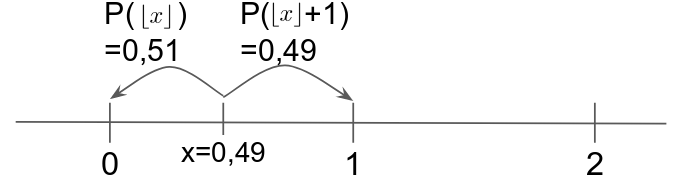
\includegraphics[width=9cm]{random_rounding}
    \caption{Exemple d'arrondi randomisé}
    \label{random_rounding}
  \end{center}
\end{figure}

On s'intéressera notamment à l'article \textit{Deep Learning with Limited Numerical Precision}\cite{gupta2015deep}, où leur démarche est d'entraîner des réseaux de neurones avec des formats restreints (en fixed-point), à faible précision, pour observer la sensibilité de l’apprentissage au mode d’arrondi.
Ils observent que lorsque la précision diminue trop, un phénomène de divergence dans l'apprentissage se dessine. Pour compenser, ils introduisent un arrondi randomisé.
Dans ce cas, ils notent qu'en fonction du mode d'arrondi, on peut observer une divergence du gradient ou une convergence (en faveur de l'arrondi randomisé).
L’idée est donc de tester cet arrondi randomisé dans d’autres cas, et finalement reproduire leurs résultats, les approfondir et les expliquer.
Une piste intéressante pour expliquer cette convergence est que l’introduction de bruit s’avère positive dans l’apprentissage de CNN : on l’ajoute donc volontairement lors de l’entraînement. De la même façon, il serait intéressant de voir dans quelle mesure le bruit induit par l’arrondi stochastique pourrait avoir un impact positif sur l’apprentissage.
\\
Avant cela, nous avons souhaité tester l’arrondi randomisé sur des procédés connus pour être numériquement instables. En l'ocurrence, le gradient conjugué, et l'attracteur de Lorenz. Le gradient conjugué est un procédé itératif permettant de résoudre des systèmes d’équations linéaires\cite{shewchuk1994introduction}.
L'attracteur de Lorenz, procédé itératif utilisé notamment en météorologie, s'avère d'autnat plus sensible à l'accumulation d'erreurs dans les calculs flottants, donc potentiellement au mode d’arrondi utilisé.
%“procédé itératif (llorenz), impact sur l’accumulation d’erreur ?”

L’implémentation de ces deux procédés a été assez complexe, puisqu’il a fallu utiliser un mode d’arrondi codé \textit{à la main} dans chaque opération.
Chaque programme est ensuite exécuté une fois avec les modes d'arrondis \textit{communs}, puis de multiples fois avec l'arrondi stochastique, dont on récolte finalement la moyenne ainsi que l'écart type des valeurs finales.

\subsubsection{Lorenz}
Les paramètres de l'attracteur de Lorenz utilisé sont $\sigma = 10$, $\rho = 28$ et $\beta = 8/3$. Aucun \textit{fine-tuning} n'a été réalisé pour l'heure sur ces paramètres : ceux par défaut ont été gardés.
On compare les valeurs testées à une exécution considérée \textit{optimale}, réalisée avec une forte précision, et on obtient les résultats de la Figure \ref{Lorenz}.\\
\begin{figure}[h]
	\begin{center}
		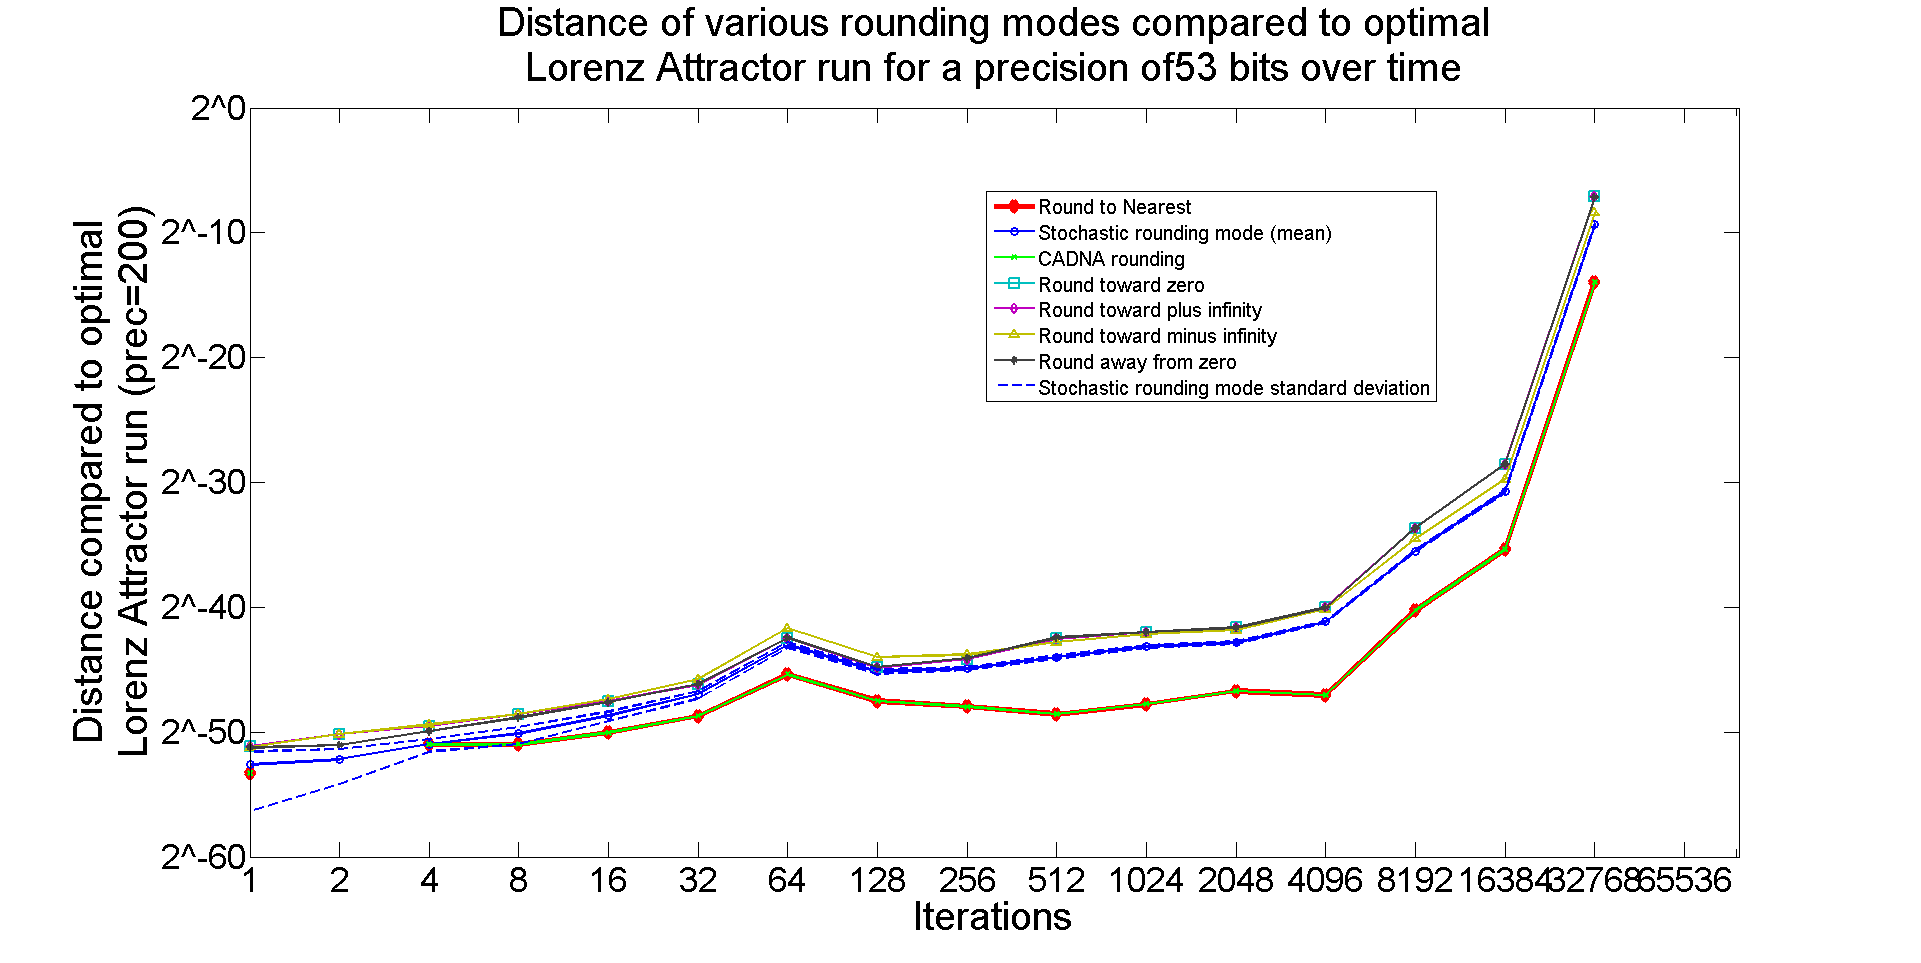
\includegraphics[width=15cm]{distance_prec=53_logx}
		\caption{Suivi de l'accumulation d'erreur en fonction du temps et du mode d'arrondi, à une précision de 53 bits (format double précision)}
		\label{Lorenz}
	\end{center}
\end{figure}
Les axes en échelle logarithmique représentent en abscisse le temps (en nombre d'itérations) et en ordonnée la distance relative à l’optimal. Plus cette distance est grande, plus on s'éloigne de la valeur \textit{correcte}.

On observe clairement les conséquences de l’accumulation d’erreur, car à mesure des itérations en perd de plus en plus en précision. 
CADNA semble fournir des résultats équivalents à ceux du mode d’arrondi standard (RNDN), dans l’ensemble plus précis que l’arrondi randomisé sur ce cas d'étude.

\subsubsection{Gradient conjugué}
Concernant le gradient conjugué, on s'est proposé de comparer les deux modes d’arrondi en fonction du nombre d’itérations, ainsi que de la précision des mantisses utilisées. Les résultats sont semblables à ceux obtenus avec Lorenz : l'arrondi au plus près semble là aussi plus efficace. En revanche, ce cas n'a pas été comparé à CADNA.
Des courbes de ces résultats seront intégrées à ce rapport une fois générées de nouveau.


%[ l’objectif était de se lancer dans les réseaux de neurones, j’ai décidé de me lancer dans l’analyse des erreurs ]
Avant de me lancer dans l’extension aux réseaux de neurones, j’ai décidé de réaliser l’implémentation de FPANR en juin dernier.

\subsection{ FPANR }
FPANR est un format d'encodage particulier, présenté dans \cite{defour2018fp}.
Le principe est d'encoder un flottant d'une manière permettant de \textbf{stocker} dans la mantisse le nombre de bits non significatifs de la valeur flottante elle-même.
On a vu qu’au cours des calculs, un nombre flottant peut être amené à accumuler du bruit. La partie de sa mantisse située du côté de bits de poids faible devient alors non signifiante.\\
L'idée d'enregistrer le nombre de bits significatifs en parallèle du flottant trouve son origine dans \textit{Significance arithmetic}\cite{goldstein1963significance}
FPANR propose un mécanisme astucieux permettant de \textbf{marquer} la partie signifiante, à l'aide d'un \textit{pattern} spécifique dans la mantisse ; l'incertitude est ainsi directement représentée, sans surcoût mémoire.
On conserve ainsi la compatibilité avec le standard IEEE754, ce qui s'avère utile pour l’allocation mémoire et l’implémentation \textit{hardware}.
\\
Le \textit{coût} engendré est un motif (indiquant la non significance) à la fin du nombre flottant ($1000....$). Ce pattern viendra remplacer des bits qui ont perdu leur sens au fil des erreurs d'arrondis. Le risque survient lorsque l'on manipule un nombre dont la précision est maximum, où FPANR se doit de \textit{tagger} le dernier bit, qui pourtant était correct. Le motif diminue donc la précision d'au plus 1 bit dans le pire des cas. % sur des process hautement dépendant de la précision, ce coût peut se révéler élevé
Autre considération, les opérations entre nombres encodés FPANR ne peuvent se faire qu’après une reconversion de ceux-ci en flottants IEEE 754, ce qui peut entraîner des conséquences en terme de performance et de temps d’exécution.
\\

Cette démarche s’architecte avec les objectifs de ma thèse en ce sens que FPANR permet de suivre la précision au fil de l’exécution.
On se propose donc d'en réaliser une intégration LLVM, afin de rendre possible l’intégration de cet encodage dans n’importe quel programme.

%L’objectif dans le cadre de ma thèse est de rendre possible l’intégration de cet encodage dans n’importe quel programme.
À cette fin, et plutôt que de redéfinir des passes LLVM \textit{à la main}, nous avons choisi de nous baser sur le travail réalisé sur Verificarlo, qui contient déjà la structure des passes nécessaires.
Cela nous a permis de gagner un temps précieux lors de la réalisation.
L’expérience est d'ailleurs un succès puisque nous avons déjà réussi à manipuler des nombres FPANR, et à les expérimenter sur quelques cas.\\
\\
Cependant, nous nous sommes heurtés à quelques difficultés, qu'il nous faut d'abord régler.
Premièrement, FPANR nécessite une conversion explicite entre un flottant IEEE 754 et un flottant FPANR. Il est donc nécessaire de transformer \textbf{toutes les entrées} des programmes cible (y compris les constantes utilisées en dur dans le code lors des calculs) pour pouvoir manipuler correctement les nombres dans le programme, et faire de même lors de \textbf{toutes les sorties} (affichage écran, écriture fichier etc). 
Pour y parvenir, plusieurs solutions ont été envisagées : la solution la plus simple est de coder à la main les conversions, à l’aide d’une librairie les contenant. Cela est pratique à court terme, mais l’objectif à moyen terme sera d’automatiser cela grâce à LLVM.
Il faudra aussi s’interroger sur le comportement à adopter lorsque le programme se heurtera à un nombre qui serait entièrement non significatif (doit-on lever ou non une exception...).
%En dernier lieu, on utilise actuellement un développement en série de Taylor d’ordre 1 pour estimer l’évolution des bits significatifs sur certaines fonctions, or il faut s’assurer que les hypothèses sous tendues sur les dérivées se vérifient en pratique.


\section{Publications en cours}
Bien que je n'ai postulé à aucune conférence dans l'immédiat, j'ai été chaleureusement encouragé par mes directeur et co-directeur à entamer la rédaction de ma démarche et des résultats obtenus au fil de l'eau, à fortiori sur l'arrondi randomisé appliqué au gradient conjugué, et à l'attracteur de Lorenz (et bientôt aux réseaux de neurones). Je dois donc finaliser et parfaire cette base afin de publier ces résultats concernant le comportement de l'arrondi randomisé sur ces processus itératifs.
\\
Dans un deuxième temps, une publication contenant les bancs de tests réalisés sur la bibliothèque FPANR, sur les SPEC\footnote{\url{https://www.spec.org/cpu2006/}} notamment, sera proposée.

\section{Planning prévisionnel}
% analyser erreurs, (identifier).
% intéresser sensibilité arrondi randomisé
% commencé à me familiariser avec les erreurs numériques (gradient, DNN)
% varier précision/mode d’arrondi, regarder comment cela impacte l’apprentissage
Lors de cette première année, j'ai commencé à me familiariser avec les erreurs numériques sur des cas tels que la descente de gradient.
J'ai pu observer le comportement et l’effet de l’arrondi randomisé sur des problèmes numériques. 
De plus, j'ai pu intégrer FPANR à LLVM, via Verificarlo, afin de tester facilement des cas généraux.
Cette partie présente les jalons restant à réaliser tout au long de ma thèse\footnote{un planning détaillé peut être consulté à la table \ref{planning} en annexe (p\pageref{planning})}.

\subsection{FPANR}
Avant de nous confronter aux codes d'érosion du littoral de GLADYS, nous tenons à confronter les outils développés jusqu'ici à des jeux de données reconnus dans le domaine : les SPEC. La publication de ces résultats occupera la fin de l'année 2018. \\
Dans un deuxième temps, on observe que FPANR peut potentiellement perdre rapidement de la précision ; envisager un modèle hybride croisé avec l'arrondi randomisé pourra s'envisager dans un deuxième temps.

\subsection{Arrondi randomisé}
La reproduction des résultats de Gupta \& al.\cite{gupta2015deep} sera au cœur de cet objectif, prolongeant l'étude sur la descente de gradient - en ce sens que l'apprentissage des réseaux de neurones se base lui aussi sur une descente de gradient. On se basera pour cela sur la bibliothèque déjà implémentée lors de la première année de thèse. Une fois ceci fait, et une fois d'autres métriques implémentées sur les cas de Lorenz et du Gradient conjugué (telles que le nombre de bits perdus dans le premier cas ou le degré de convergence dans le second), s'atteler à leur publication.

\subsection{GLADYS}
% Confrontation
% automatic differentiation, verificarlo, cadna, qui sont d’autres outils dans le domaine, qui pourront me servir de repères
%l’objectif de ma thèse c’est de voir un vrai code. aidé par des experts qu’on a dans la région, qui sont compétents sur le sujet : les modèles et simulations de Gladys.
Une fois notre outil confronté aux initiatives existantes, qui auront servi de repères, la vocation centrale de la thèse ACSEL se matérialisera en l'appliquant aux modèles de prédiction d'érosion du littoral de GLADYS. Les problématiques traitées par cette communauté ont une réelle portée sociétale et écologique (montée des eaux, immobilier, tourisme, etc), qui est une motivation supplémentaire à contribuer à ce travail.
% Application aux modèles de prédiction d’érosion du littoral de GLADYS
%Récolte de statistiques sur les programmes par méthode de Monte Carlo
Pour cela, je pourrai m'appuyer sur les experts que nous avons dans la région, compétents sur le sujet.
Concernant le choix du modèle et de la simulation à étudier, un rapport de critères sera fourni à Frederic Bouchette, référent côté Gladys, pour lesdites simulations, et membre du CSI. Après étude de ce dernier et discussions, des simulations seront choisies en fonction de leurs caractéristiques pour servir de sujet d'étude à cette thèse.
On s'appliquera à étudier des simulations qui présentent potentiellement des erreurs numériques, afin de valider notre démarche tout en ayant un réel apport auprès des chercheurs de cette communauté.
\\
Ensuite, on se propose de récolter les statistiques sur les programmes étudiés, notamment par méthode de Monte Carlo.
Enfin, on procèdera à l'extraction de l'information pertinente de ces statistiques, en utilisant des méthodes de Data Mining (Random Forest...).
Ces informations seront en dernier lieu délivrées dans un format intelligible à l'utilisateur.
% Récolte de statistiques sur les programmes par méthode de Monte Carlo
%Application aux modèles de prédiction d’érosion du littoral de GLADYS

%finalement, l’idée sera d’extraire l’information pertinente de ces statistiques, avec des méthodes de Data Mining (Random Forest)
%et de la délivrer à un format intelligible à l’utilisateur, via des indicateurs (voire des recommandations).
%Pour un plus large champ d’application  ==> LLVM

% (; et de le faire de manière assez générique pour que cela s’applique aux modèles de gladys - mais pas uniquement.
% (faire un outil qui pourra être applicable dans différents domaines ; on envisageait d’utiliser l’outil de compilation libre LLVM, pour réaliser des passes automatiques dans les implémentations des modèles afin d’en extraire de l’information par exemple)
% analyse descriptive)

\subsection{Rédaction}
Tout au long de ma thèse, et à fortiori durant la dernière année, il sera indispensable de commencer à rédiger la thèse en elle-même.
Le rythme de rédaction devra aller croissant à partir de maintenant. Je pourrais me baser sur la capitalisation d'informations déjà réalisée notamment sur l'arrondi randomisé, ainsi que sur certains éléments présentés dans le présent documents.

\section{Difficultés rencontrées}
Il m'a été difficile de déterminer, d'un point de vue \textit{scientifique}, quels résultats étaient significatifs (ou non), à fortiori lors de l'étude de l'arrondi randomisé. J'aurais aimé tester davantage de cas mettant en valeur l'arrondi randomisé, à fortiori des cas où son impact est significatif.
Je n'étais pas certain que les résultats obtenus sur les cas étudiés étaient \textit{suffisants}, dans le sens \textit{probants} car utiles à la communauté scientifique. Cela a quelque peu miné mon avancement et soulevé de nombreux doutes. Désormais, une meilleure connaissance de l'état de l'art me permets d'être plus confiant à ce niveau.\\
Dans un deuxième registre, commencer à rédiger l'article sur l'arrondi randomisé (et le faire régulièrement au fil de mes progrès) a été toute une procédure à mettre en place pour moi : je n'avais pas l'habitude de formaliser aussi explicitement ma pensée sur un projet, en l'ocurrence de recherche, aussi cela m'a pris du temps avant d'y parvenir.\\
Dans un dernier temps, j'ai observé une difficulté à prendre du recul sur le travail, et une tendance à s'enfoncer sur des points de blocage, sans parvenir à formuler des appels à l'aide qui auraient permis de débloquer rapidement ces points. A l'avenir, des efforts doivent être mis en œuvre pour consulter plus régulièrement les intervenants aptes à résoudre mes éventuels problèmes, qu'ils soient d'ordre technique ou théoriques.
%21. Questions
%différence DSA (CESTAC) / MCA :
%DSA : on run chaque opération N fois
%MCA, on run tout le programme de multiples fois

%“que ça en un an?”
%==> passage du monde de l’industrie à la recherche qui m’a demandé de l’adaptation ; maintenant je pense que je suis sur la bonne voie

%25. Difficultés
%- Obtention résultats arrondi randomisé\\
%-- Qu’est-ce qui est significatif? \\
%-- Problématique intrinsèque à la démarche de recherche\\
%-- les cas d’utilisations mettant en valeur l’arrondi randomisé : j’aurais du en avoir plus\\
%-- l’article aurait pu être publié selon Bijan, et non selon David : or moi la partie DNN m’intéresse beaucoup (voire de m’orienter là dedans plus tard) donc je tenais à l’intégrer à l’article et donc à continuer à chercher\\
%- Perte massive de données au début de l’été 2018\\
%- Difficulté de rédaction de l’article\\
%-- Méthode scientifique autant que de rédaction complexe à mettre en oeuvre\\
%- Manque de recul, désorientation quant à la méthode de travail\\
%-- Désormais résolu, efforts canalisés et bien aiguillés\\

\bibliography{bibliography/bibCSI}{}
\bibliographystyle{plain}

\section{Annexe : Planning détaillé}
\begin{table}[h]
	\caption{Planning détaillé - 2018}
	\label{planning}

	\centering
	%\begin{center}
	%\begin{tabular}{c|c|p{20em}}
	\begin{tabular}{c|p{25em}}
		\hline
			%semaines 39-40 & 24/09 - 03/10 & Planification détaillée du projet de thèse, capitalisation avancement dans un rapport \\ 
		 semaine 40 (Oct-18) & Planification détaillée du projet de thèse, capitalisation avancement dans un rapport \\ 
		 & \\
		 	%semaines 40-41 & 04/10 - 12/10 & Création de la bibliothèque de conversion pour FPANR, intégration à Verificarlo, rédaction des tests correspondants \\
		 semaine 41 (Oct-18) & Création de la bibliothèque de conversion pour FPANR, intégration à Verificarlo, rédaction des tests correspondants \\
		 & \\
		 	%semaine 42 		& 14/10 - 19/10	& Participation à la formation doctoriales \\
		 semaine 42 (Oct-18)	& Participation à la formation doctoriales \\
		 & \\
		 	%semaine 43			& 22/10 - 26/10 & Familiarisation avec la documentation complète des SPEC, afin de manipuler leur jeux de données \\
		 semaine 43	(Oct-18) & Familiarisation avec la documentation complète des SPEC, afin de manipuler leur jeux de données \\
		 & \\
		 	%semaines 43-45 & 22/10 - 09/11 & En parallèle, travailler sur l'automatisation de la conversion des entrées/sorties  \\
		 semaines 43-45 (Oct-18) & En parallèle, travailler sur l'automatisation de la conversion des entrées/sorties  \\
		 & \\
		 	%semaines 44-45	&	29/10 - 06/11 & Application de FPANR/LLVM à un jeu de données simple des SPEC, pour tester la faisabilité de la démarche \\
		 semaine 44 (Nov-18) & Prise en main des SPEC, compilation, exécution et maitrise d'un cas d'exemple \\
		 & \\
		 semaine 45 (Nov-18) & Application de FPANR/LLVM à quelques jeux de données simples des SPEC, pour tester la faisabilité de la démarche \\
		 & \\
		 semaine 46 (Nov-18) & Appréciation de la démarche, retour critique sur les fonctionnalités et les spécifications de la librairie FPANR \\
		 & \\
		 semaines 47-48 (Nov-18) & Compilation et exécution des jeux de données SPEC via FPANR/LLVM \\
		 & \\
		 semaine 49 (Dec-18) & Récolte et formatage des résultats \\
		 & \\
		 semaines 50-51 (Dec-18) & Rédaction et publication des résultats FPANR \\
		 \end{tabular}
	%\end{center}
\end{table} 

\begin{table}[h]
	\caption{Planning détaillé - 2019/2020}
	\centering
	%\begin{center}
	%\begin{tabular}{c|c|p{20em}}
	\begin{tabular}{c|p{22em}}
		\hline
		 semaines 1-4 (Jan-19) & Retour sur l'arrondi randomisé, regénération pertinente des résultats du gradient et de Lorenz \\
		 & \\
		 semaines 5-8 (Feb-19) & Reproduction des résultats de Gupta : entraînement de réseaux de neurones avec un arrondi randomisé (+ bibliographie) \\
		 & \\
		 semaines 9-13 (Mar-19) & Perfection des résultats, rédaction article \\
		 & \\
		 semaines 14-17 (Apr-19) & Rédaction spécifications programmes Gladys + intégrations des retours de la revue par les pairs \\
		 & \\
		 semaines 18-21 (May-19) & Prise en main des simulations de Gladys, compréhension fonctionnement, fil d'exécution \\
		 & \\
		 semaines 22-26 (Jun-19) & Modélisation des métriques et indicateurs à mettre en place \\
		 & \\
		 semaines 27-30 (Jul-19) & Mise en place des indicateurs, début d'application de notre outil \\
		 & \\
		 semaines 31-34 (Aug-19) & Itérations sur les simulations, tests et récolte de données \\
		 & \\	
		 semaines 36/2019-22/2020 (19-20) & Rédaction thèse \\
		 & \\
		 semaines 36/2019-09/2020 (19-20) & En parallèle, exportation des indicateurs, automatisation de l'information à l'utilisateur, conclusions sur ce cas d'étude \\
		 & \\
		 semaines 10-22 (Mar-Jun - 20) & Valorisation, contribution à des colloques, séminaires \\
		 & \\
		 semaines 23-35 (Jul-Sept - 20) & Préparation thèse, soutenance de thèse
	\end{tabular}
	%\end{center}
\end{table}


\end{document}
